% !TEX encoding = UTF-8
% !TEX TS-program = pdflatex
% !TEX root = apprendimento_automatico.tex
% !TEX spellcheck = it-IT
\section{Lezione 5 VC-Dimension e VC-Confidence}\label{lezione-5-vc-dimension-e-vc-confidence}

\subsection{Esempi di spazi delle ipotesi}\label{esempi-di-spazi-delle-ipotesi}

Seguono alcuni esempi di spazi per le ipotesi nei problemi di
apprendimento supervisionato, cioè quei problemi in cui si vuole
stabilire se un elemento \emph{x} appartiene o meno ad una classe.

\subsubsection{Iperpiani in R2}\label{iperpiani-in-r2}

\textbf{Iperpiano}: dato uno spazio a \emph{n}-dimensioni, un iperpiano
per quello spazio è un sottospazio di dimensione \emph{n-1}. Quindi gli
iperpiani in R2 sono tutte le rette del piano.

Lavorando in R2 lo spazio delle istanze è definito come:

\begin{quote}
X = \{x \textbar{} x ∈ R2\}.
\end{quote}

Mentre lo spazio delle ipotesi è dato dalle dicotomie indotte da
iperpiani in R2, cioè da tutte le possibili divisioni del piano.

\begin{quote}
H = \{f(w,b)(x) \textbar{} f(w,b)(x) = sign(w * x + b), w ∈ R2, b ∈ R\}
\end{quote}

Così facendo vengono prese in considerazione tutte le rette che dividono
R2 in due parti in modo che da una parte l'ipotesi valga 1 e dall'altra
-1.

\subsubsection{Dischi in R2}\label{dischi-in-r2}

Sempre in R2 è possibile considerare come spazio delle ipotesi tutte le
dicotomie indotte da disci in R2 e centrati nell'origine.

\begin{quote}
H = \{fb(x) \textbar{} fb(x) =
sign(\textbar{}\textbar{}x\textbar{}\textbar{}2 - b), w ∈ R2, b ∈ R\}
\end{quote}

Il che vuol dire che all'interno del disco le ipotesi valgono -1 mentre
al di fuori valgono 1.

\subsubsection{\texorpdfstring{Congiunzione di \emph{m} letterali
positivi}{Congiunzione di m letterali positivi}}\label{congiunzione-di-m-letterali-positivi}

Lo spazio delle istanze questa volta è dato da tutte le stringhe di
\emph{m} bits

\begin{quote}
X = \{s \textbar{} s ∈ \{0,1\}m\}
\end{quote}

Lo spazio delle ipotesi è dato da tutte le sentenze logiche che
riguardano i letterali positivi l1,l2,\ldots{},lm (li è vero se
l'\emph{i}-esimo bit è 1) e che contengono solo l'operatore ⋀.

\begin{quote}
H = \{ f\{i1,\ldots{},ij\}(s) \textbar{} f\{i1,\ldots{},ij\} (s)
equivale a li1 ⋀ li2 ⋀ \ldots{} ⋀ ij, \{i1\ldots{}ij\} sottoinsieme di
\{1..m\}\}
\end{quote}

\subsection{Misurare la complessità dello spazio delle
ipotesi}\label{misurare-la-complessituxe0-dello-spazio-delle-ipotesi}

Considerato un determinato spazio delle ipotesi \emph{H}, questo
contiene sempre:

\begin{itemize}
\tightlist
\item
  L'\textbf{ipotesi più specifica}: ipotesi più stretta, consistente con
  i dati, nell'esempio del disco è il disco più stretto in grado di
  contenere tutti i punti negativi.
\item
  L'\textbf{ipotesi più generale}: quella più grande, consistente con i
  dati, sempre nell'esempio del disco, è quello del disco più grande
  possibile e che non contiene punti positivi.
\end{itemize}

\textbf{shattering}: (frammentazione), dato \emph{S} sottoinsieme dello
spazio delle istanze, si dice che \emph{S} è frammentato dallo spazio
delle ipotesi \emph{H} se:

\begin{quote}
∀ S' ⊆ S, ∃ h ∈ H, tale che ∀x in S, h(x) = 1 se e solo se x appartiene
a S'.
\end{quote}

Cioè \emph{H} realizza tutte le possibili dicotomie di \emph{S}.

\emph{H} frammenta un certo insieme \emph{S} se è possibile trovare un
iperpiano che raccoglie tutti i punti dell'insieme \emph{S}. Ovvero per
tutte le dicotomie di \emph{S} esiste un iperpiano che riesce a
realizzarle.

\subsubsection{VC (Vapnik-Chervonenkis)
Dimension}\label{vc-vapnik-chervonenkis-dimension}

La VC-Dimension è la dimensione di uno spazio delle ipotesi \emph{H}
definito su uno spazio delle istanze \emph{X} ed è data dalla
cardinalità del sottoinsieme più grande frammentato da \emph{H}.

\begin{quote}
VC(H) = max(S ⊆ X)\textbar{}S\textbar{} tale che H frammenta S

VC(H) = ∞ se S non è limitato
\end{quote}

Ad esempio nello spazio delle ipotesi dato dagli iperpiani su R2:

Se nello spazio delle istanze ho 2 punti, questo viene frammentato da
\emph{H}, perché posso sempre trovare una retta che riesce a realizzare
tutte le possibili dicotomie di due punti su un piano.

Se nello spazio delle istanze ho 3 punti, riesco comunque a realizzare
tutte le dicotomie.

Se nello spazio delle istanze ho 4 punti qualsiasi non si riesce a
trovare un iperpiano che realizza la dicotonomia, quindi \emph{VC(H) =
3}.

Segue che, prendendo uno spazio delle ipotesi di cardinalità finita si
ha che:

\begin{quote}
VC(H) ≤ log2(\textbar{}H\textbar{})
\end{quote}

Questo perché per ogni \emph{S} frammentato da \emph{H}, abbiamo
\emph{\textbar{}H\textbar{} \textgreater{}= 2\textbar{}S\textbar{}},
cioè per ogni dicotomia in \emph{S} esite un ipotesi in \emph{H} che la
realizza, ovvero devono essere disponibili in \emph{H} tante ipotesi
quanti sono le dicotomie in \emph{H}.

Scegliendo un \emph{S} tale che \emph{\textbar{}S\textbar{} = VC(H)}, si
ottiene \emph{\textbar{}H\textbar{} \textgreater{}= 2VC(H)}, prendendo
il logaritmo si trova quello che si stava cercando, ovvero \emph{VC(H)
\textless{}= log2(\textbar{}H\textbar{})}.

\textbf{Dal libro}:

Se un dataset contiene \emph{N} elementi, questi \emph{N} elementi
possono essere etichettati con degli 0 e 1 in \emph{2N} modi diversi.

Se per ognuno di questi modi è possibile trovare un ipotesi \emph{h ∈ H}
che separa tutte le istanze negative da quelle positive allora si dice
che \emph{H} frammenta il dataset \emph{N}. Il che vuol dire che il
dataset \emph{N} può essere appreso con un errore empirico nullo.

Il massimo numero di punti che possono essere frammentati da \emph{H} è
detto \emph{VC(H)} e fornisce una misura della capacità di \emph{H}.

\subsection{Bound sull'errore di
generalizzazione}\label{bound-sullerrore-di-generalizzazione}

Considerando un problema di apprendimento binario, con:

\begin{quote}
Training set S=\{(xi,yi)\}i=1\ldots{}N

Spazio delle ipotesi H=\{h (x)\}
\end{quote}

Supponendo di avere un algoritmo di apprendimento \emph{L} che
restituisce l'ipotesi \emph{h*(x)} che minimizza l'errore empirico su
\emph{S} espresso come \emph{erroreS(h(x))}.

È possibile derivare un bound (limite superiore) per l'errore ideale o
errore di generalizzazione, valido con probabilità \emph{(1 - δ)} con
\emph{δ} piccolo a piacere:

\begin{quote}
erroreD(h(x)) ≤ erroreS(h(x)) + g(N, VC(H), δ)
\end{quote}

Il primo termine \emph{erroreS(h(x))} dipende dall'ipotesi restituita
dall'algoritmo di apprendimento L.

Il secondo termine \emph{g(N, VC(H), δ)} non dipende da \emph{L}, ma dal
numero di esempi di training utilizzati (inversamente proporzionale),
dalla \emph{VC-dimension} (direttamente proporzionale) e dalla
confidenza, ovvero dal termine \emph{δ}.

Il termine \emph{g(N, VC(H), δ)} viene anche chiamato
\textbf{VC-confidence} e risulta essere monotono rispetto al rapporto
\emph{VC(H)/N}.

\subsection{Structural Risk Minimization
(SRM)}\label{structural-risk-minimization-srm}

Approccio per la scelta dello spazio delle ipotesi proposto da Vapnik
che cerca di trovare un compromesso tra l'errore empirico e la
VC-Confidence.

Si considerano spazi delle ipotesi sempre più piccoli H1  H2  \ldots{}
 Hn tali che VC(H1) ≤ VC(H2) ≤ \ldots{} ≤ VC(Hn)

Si seleziona lo spazio delle ipostesi Hi che ha il valore del bound
sull'errore di generalizzazione più piccolo.

\begin{figure}[htbp]
\centering
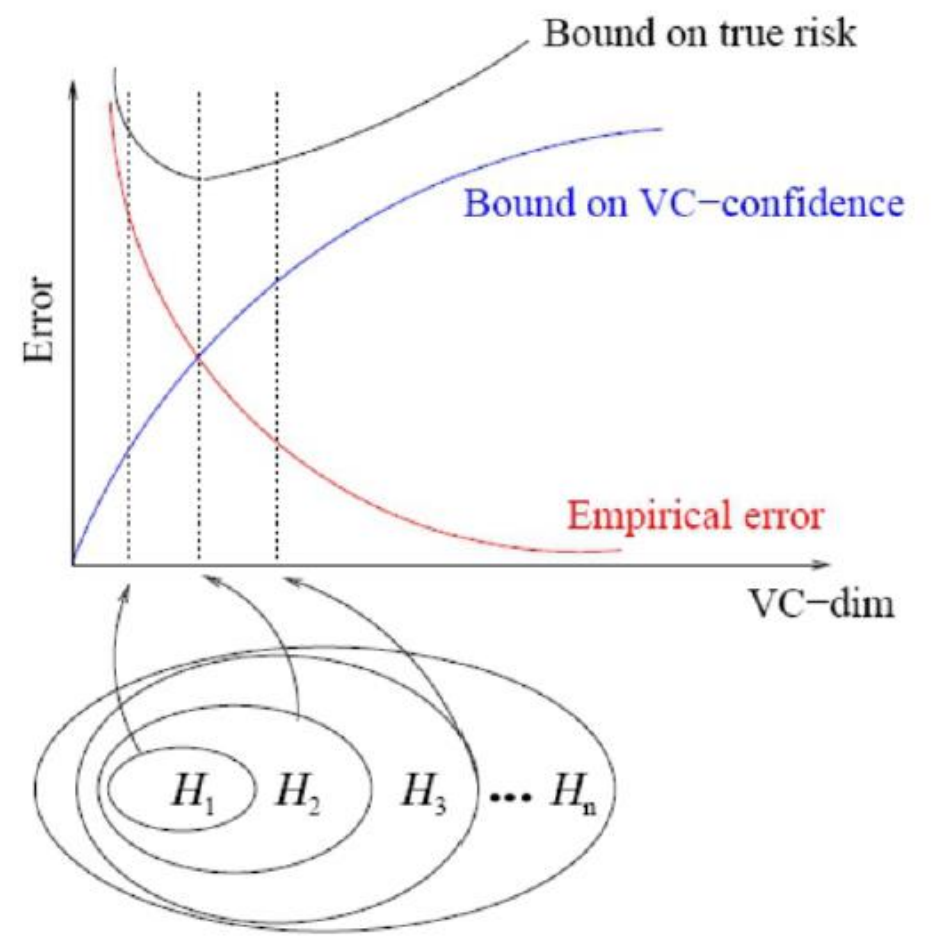
\includegraphics{./notes/immagini/l5-srm.png}
\caption{}
\end{figure}
